\chapter{Entwurf und Implementierung}
\label{cha:implementierung}

\todo{Kapitel-Einleitung}

\section{Modularer Architektur-Vorschlag}

%Komponenten des Brokers.
%
%
%In der CMP: Polling oder Notification?
%
%Was löst eine Aktion aus?
%- Monitoring der Services
%- Änderung der Umgebung
%- User-Aktion
%- Ergebnis einer anderen Policy

\begin{figure}
	\centering	
%	\def\svgwidth{0.95\textwidth}
%	{\tiny
%	\includesvg{images/broker-cycle}}
	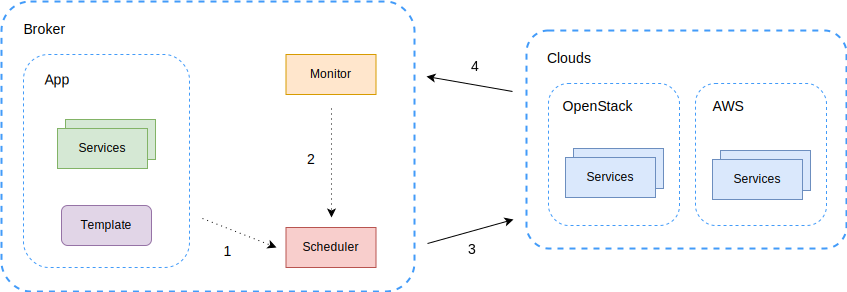
\includegraphics[width=\linewidth]{images/broker-cycle}
	\caption{Arbeitsweise des Multi-Cloud-Brokers als Zyklus: (1) Sammeln der Meta-Informationen aller Cloud-Provider, (2) Sammeln der Laufzeitinformationen der Anwendungen, (3) Sammeln der SLAs, (4) Nutzeränderungen: Neue Anwendungen oder Anpassung von SLAs, (5) Optimierungsplanung, (6) Planausführung auf den Cloud-Infrastrukturen}
	\label{fig:cycle}
\end{figure}

%Zyklus\autoref{fig:cycle}:

%\begin{description}
%	\item[Nummerierte Aufzählung]~\par
\begin{enumerate}
	
	\item Sammeln der Meta-Informationen alle Cloud-Provider
	\begin{enumerate}
		\item Kapazität (CPU, RAM, HDD, Network)
		\item Features (Verschlüsselung, CUDA, …)
		\item Geo-Lokation 
		\item Preis
	\end{enumerate}
	
	\item Sammeln der Laufzeitinformationen der PaaS/Anwendungen
	\begin{enumerate}
		\item Auslastung
		\item Fehler
		\item Ausfälle
	\end{enumerate}
	
	\item Sammeln der SLAs
	\begin{enumerate}
		\item Policy-Definitionen
		\item Policy-Konfiguration
		\item Placement-Algorithmen
	\end{enumerate}
	
	\item Neue Anwendung/Änderung eines SLA
	
	\item Optimierung
	\begin{enumerate}
		\item Feste Vorgaben (Geo, Backup)
		\item Weiche (Preis, Latenz, Verfügbarkeit)
	\end{enumerate}
	
	
	\item Ausführung
	\begin{enumerate}
		\item Netzwerkkonfiguration
		\item Allokation/De-Allokation von Ressourcen
		\item Deployment
		\item Migration
		\item Logging/Benachrichtigung
		\item Backup
	\end{enumerate}
	
\end{enumerate}

\section{Brokering}


%https://de.wikipedia.org/wiki/Constraintprogrammierung
%https://de.wikipedia.org/wiki/Scheduling

%entailing multiple constraint satisfaction (MCS)
%
%\todo{Schaubild, was wird wann gematcht}
%% Pseudocode des Algorithmus, wie in Meryn
%
%Kostenoptimierung
%
%Preisentwicklung? 
%
%Migration je nach Tageszeit? 
%
%Kosten der Datentransfers 
%
%Subscription On-Demand/Monthly/Yearly 
%
%Kompliziert durch undurchsichtige Staffelpreise
% https://www.rightscale.com/blog/cloud-cost-analysis/aws-vs-azure-vs-google-cloud-pricing-compute-instances

%https://www.rightscale.com/blog/cloud-cost-analysis/comparing-cloud-instance-pricing-aws-vs-azure-vs-google-vs-ibm

%
%Cost Calculators 
%
%http://go.appscale.com/cloud-cost-calculator-help 
%
%https://github.com/ifosch/accloudtant 
%
%https://awstcocalculator.com/# 
%
%Kosten: Rechenzeit und Bandbreite (außerhalb einer Cloud) also gegenläufiges Ziel zu Portabilität und Ausfallsicherheit, denn die geringsten Kosten fallen bei dem Betrieb in einer einzelnen Cloud eines Providers an.
%i) providers’ pricing models, (ii) application’s communication patterns and (iii) distribution of nodes over providers.
%https://www.google.de/url?sa=t&rct=j&q=&esrc=s&source=web&cd=1&ved=0ahUKEwju27vHs6DZAhUCWRQKHRv7BEcQFggrMAA&url=http%3A%2F%2Fwww.mikesmit.com%2Fwp-content%2Fpapercite-data%2Fpdf%2Fcloud2012.pdf&usg=AOvVaw3e6yhHYmhWBbIxtr7MqkuX


\section{Testanwendung: Hyrise-R}

Hyrise\footnote{\url{https://hpi.de/plattner/projects/hyrise.html}} ist eine In-Memory-Forschungsdatenbank der Fachgruppe \emph{Enterprise Platform and Integration Concepts (EPIC)} am Hasso-Plattner-Institut \cite{grund:2010:hyrise}. Die Datenbank teilt sich einige Eigenschaften mit \emph{SAP HANA}\footnote{\url{https://www.sap.com/products/hana.html}}: Ein \emph{Delta Store}, spaltenorientierte Speicherung, Wörterbuchkodierung und weitere Komprimierungstechniken sowie den \emph{Insert-Only}-Ansatz und Partitionierung. Herausragend ist die OLAP-Performance, enthalten sind aber auch Optimierungen für OLTP-Aufgaben.

Hyrise-R ist eine Erweiterung des Basisprojektes um Replikation \cite{schwalb:2015:hyrise-r}. Es folgt dabei dem \emph{Scale-Out}-Ansatz: Alle schreibenden Operationen werden auf einem einzigen \emph{Master-Node} durchgeführt. Dessen Datensatz wird in weniger als einer Sekunde (\emph{lazy}) mit beliebig vielen \emph{Replica-Nodes} abgeglichen. Diese Spiegelungen bearbeiten alle reinen Leseanfragen und machen den Verbund so skalierbar, siehe \autoref{fig:hyrise-r}. Nach dem \emph{CAP-Theorem} sind Verfügbarkeit und Partitionstoleranz hier also wichtiger als Konsistenz. 

\begin{figure}[ht]
	\centering
	\def\svgwidth{0.9\textwidth}
	\textsf{
	\includesvg{images/hyrise-r}}
	\caption{Verteilte \emph{Hyrise-R}-Architektur mit getrennter Verarbeitung von Lese- und Schreibanfragen. Der Master-Knoten dient als \emph{Single Source of Truth}. Zur Leistungssteigerung übernehmen Spiegelserver die Beantwortung der meisten Leseanfragen. Kleinere Inkonsistenzen werden dabei in Kauf genommen. Nicht im Bild ist der Dispatcher zur Anfrageverteilung. Aus \cite{ssiclops:d42:experiments-measurements}.}	
	\label{fig:hyrise-r}
\end{figure}

Durch die verteilte Architektur ist Hyrise-R ein potenzieller Kandidat als Testanwendung innerhalb der Multi-Cloud-Umgebung. Einige \emph{SSICLOPS}-Teilprojekte untersuchten bereits Zuverlässigkeit, Performance, Datensicherheit und Vertraulichkeit in einer privaten OpenStack-Föderation \cite{ssiclops:d23:security-extensions, ssiclops:d42:experiments-measurements, bastian:2017:openstack-policies}.

Im Rahmen dieser Arbeiten sind einige Infrastrukturteile als Code veröffentlicht: So existiert zum Beispiel eine Docker-Teststellung mit grafischem Cluster-Manager, um die Performance bei verschiedenen Replikationsstufen zu prüfen. Diese Infrastruktur wurde in mehreren Studienarbeiten weiter angepasst, um Hyrise-R-KVM-Images in OpenStack bereitzustellen \cite{eschrig:2016:ssiclops-masterproject, maschler:2017:ssiclops-masterproject}.

Um als Testanwendung über mehrere Cloud-Ebenen zu dienen, sollte Hyrise-R auf den verbreiteten Hypervisoren, IaaS- und CaaS-Providern ausführbar sein. Aufgrund der Softwarestruktur -- als eigenentwickelte \emph{Low-Level-C++-Anwendung} --  eignet Hyrise-R sich nicht direkt\footnote{\url{https://cloud.google.com/appengine/docs/flexible/custom-runtimes/}} als Testanwendung für die PaaS-Integration. Hierfür nutzen wir andere Standardsoftware, die auf den üblichen PaaS-Sprachen wie Java, Python oder Node.js aufbauen.

Hyrise-R ist von Anfang an für die Skalierung über externe Broker konzeptioniert. Die bisherigen Arbeiten haben \emph{Standalone-Cluster-Manager} umgesetzt, erst für Docker und später für OpenStack\footnote{\url{https://github.com/DukeHarris/hyrise_rcm}}\footnote{\url{https://github.com/SSICLOPS/openstack-testbed-vm}}. Die nötigen Clusterinformationen werden Hyrise-Instanzen direkt beim Start als Parameter übergeben. Variablen zur Laufzeitumgebung müssen während des Deployments vom Broker ausgefüllt werden: Konkret benötigt Hyrise einen TCP-Port und eine eindeutige Knoten-ID. Über ihre ID registrieren sich Knoten am Dispatcher. Hierzu benötigen sie dessen IP-Adresse und Port -- der Dispatcher muss also immer als Erstes in einem Cluster bereitstehen. Erst dann können Start und Registrierung des Masters erfolgen. Plattformunabhängig ergeben sich folgende Startskripte für einen Hyrise-R-Cluster:

\begin{description}
	
\item[{[1]} Dispatcher] einmal pro Cluster, zentrale Lastverteilung für alle Anfragen
	
\begin{minted}{jinja}
./dispatcher {{dispatcher.port}} settings.json
\end{minted}
	
\item[{[1]} Master] einmal pro Cluster als \emph{Single-Source-of-Truth}, bearbeitet alle Schreibanfragen, gekennzeichnet durch \emph{nodeId=0}
	
\begin{minted}{jinja}
./hyrise \
  --dispatcherurl={{dispatcher.ip}} \
  --dispatcherport={{dispatcher.port}} \
  --nodeId=0 \
  --port={{master.port}}
\end{minted}

\item[{[0-n]} Replica] optional, beliebig viele Instanzen pro Cluster zur Entlastung des Master-Knotens bei Leseanfragen

\begin{minted}{jinja}
./hyrise \
  --dispatcherurl={{dispatcher.ip}} \
  --dispatcherport={{dispatcher.port}} \
  --nodeId={{replica.id}} \
  --port={{replica.port}}
\end{minted}
	
\end{description}

In vorherigen Projekten entwickelte Images für virtuelle Maschinen laufen auf der verbreiteten Hypervisorkombination aus QEMU und KVM. Die Erstkonfiguration erfolgte bisher über direkte SSH-Kommandos an die gestartete virtuelle Maschine. Dies erfordert die Konfiguration von SSH in den VMs und die Verwaltung von Schlüsseln in der CMP. Zusätzlich entsteht eine Wartezeit zwischen VM-Startkommando und Erstkonfiguration, die vorherige Projekte durch Polling noch ausdehnten. Eine elegantere Lösung ist \emph{cloud-init}: Die CMP füllt ein Konfigurationstemplate und schickt es direkt im Startkommando an den Infrastruktur-Provider. Dieser führt das Skript sofort ohne weitere Wartezeit aus.

Auch Docker-Images existieren bereits\footnote{\url{https://github.com/hyrise/hyrise-v1/tree/feature/docker}}, wurden aber seit 2015 nicht aktualisiert: Docker, diverse Abhängigkeiten und Hyrise selbst wurden in der Zwischenzeit weiterentwickelt. Innerhalb eines Clusters sollten alle Knoten dieselbe Hyrise-Version ausführen. Daher aktualisieren wir Dispatcher und Hyrise auf Basis des aktuellsten Hyrise-NVM-Branches\footnote{\url{https://github.com/janmattfeld/dispatcher/tree/docker}}\footnote{\url{https://github.com/janmattfeld/hyrise_nvm/tree/feature/docker}}.

Die Aktualisierung enthält das aktuelle Docker-Basis-Image Ubuntu 16.04. Wir integrieren außerdem korrekte Metadaten und Dokumentation zur Imageerstellung und Ausführung. Einige eingebundene Git-Submodule wurden in der Zwischenzeit verschoben oder existieren nicht mehr -- die verwendete CSV-Bibliothek muss zum Beispiel ausgetauscht werden. Dies erfordert kleinere Änderungen am Quellcode. Genauso wie neue \emph{Non-Uniform-Memory-Access-Funktionen (NUMA)}: Die Funktion \emph{membind} erfordert erweitere Rechte. In einem Standard-Docker-Container sind diese aber nicht vorhanden. Der neue Startparameter \mbox{\emph{-\,-disable\_membind}} deaktiviert die speziellen NUMA-Funktionen. Unsere Images laufen daher auch in Container-Laufzeitumgebungen der Public-Cloud-Provider.

Das Image ist zum Produktivbetrieb gedacht: Docker Build entfernt nach dem Image-Erstellungsprozess alle Abhängigkeiten, die zum Betrieb nicht notwendig sind. So reduziert sich die Image-Größe von über 500 auf weniger als 300\,MB -- entsprechend verkürzt sich die Startzeit. Enthalten ist außerdem eine Beispieldatenbank, die wir später als Benchmark und initialen Funktionstest nutzen werden. Gemessen wird also nicht die Synchronisationszeit der Hyrise-R-Lösung, sondern die Skalierungsfähigkeiten der verwendeten Cloud-Lösungen und Orchestrierungstechniken. Wir setzen außerdem pragmatische Startparameter für Hyrise-R auf Docker: \emph{-\,-corecount=2} \emph{-\,-disable\_membind}. Die neuen Images sind zur leichteren Integration auf Docker Hub veröffentlicht\footnote{\url{https://hub.docker.com/r/hyrise/dispatcher/}}\footnote{\url{https://hub.docker.com/r/janmattfeld/hyrise_r/}}. Um auch zukünftige Weiterentwicklungen von Hyrise nutzen zu können, automatisiert ein neues Makefile Docker-Build-Voränge und den Realease auf Docker Hub.

Aus der bisher losen Sammlung von Quellcode, Shell-Skripten und Makefiles in mehreren GitHub-Repositorys haben wir eine nachhaltige Pipeline zur automatisierten Image-Erstellung für verschiedene Infrastrukturen entwickelt\footnote{\url{https://github.com/janmattfeld/hyrise_nvm/commit/cfe3aa8}}. Ausführungsumgebung, Programm, Testdaten und Konfiguration werden flexibel integriert -- Hyrise-R eignet sich nun als Testanwendung für den Multi-Cloud-Broker.

Als Weiterentwicklung zu den bisherigen Hyrise-R-Arbeiten soll der Broker nicht nur nach Leistungsanforderungen skalieren, sondern auch SLAs und Geostandorte beachten sowie diverse Infrastrukturanbieter nutzen.


\section{Private-Cloud: OpenStack-Testbed}

Als Beispiel für eine Private-Cloud -- als Teil unseres Multi-Cloud-Setups -- soll OpenStack dienen. Es ist das populärste Open-Source-Projekt um eigene Infrastruktur als Service aufzubauen. Gesponsert wird es von Großunternehmen wie \emph{HPE}, \emph{IBM}, \emph{Canonical}, \emph{Red Hat} und anderen.

OpenStack setzt sich aus verschiedenen Teilprojekten zusammen, die jeweils einen Dienst entwickeln und bereitstellen. Ein Minimal-Setup besteht aus \emph{Nova} (Computing), \emph{Key\-stone} (Authentifizierung), \emph{Neutron} (Netzwerk) und \emph{Glance} (Images). Verbreitet sind außerdem \emph{Cinder} (Blockspeicher) und \emph{Horizon} (Dash\-board). Diese sollen auch in unserem Beispiel genutzt werden. Denkbar ist darüber hinaus die Integration eines Container-Dienstes. Der Zugriff auf die Infrastruktur erfolgt entweder über das Dashboard, Kommandozeilentools oder eine REST-API.

Grundsätzlich wäre auch der Aufbau einer OpenStack-Föderation wie in \emph{SSICLOPS} denkbar \cite{ssiclops:2015:d6.1-project-presentation}. Föderierte Cloud-Architekturen teilen sich zentrale Komponenten, in OpenStack mindestens den Authentifizierungsservice \emph{Keystone}. Je nach Föderationsvariante (\emph{Cells}, \emph{Regions}, \emph{Availability Zones} oder \emph{Host Aggregates}) sind auch Dienste wie Dashboard oder Speicher nur einmal vorhanden. Diese Architektur reduziert Fixkosten, erfordert allerdings spezielle Anpassungen innerhalb der Cloud. Auch gehen einige Vorteile wie Ausfallsicherheit und Unabhängigkeit der zentralen Dienste wieder verloren. Eine Kombination mit weiteren Cloud-Providern im Rahmen unseres Multi-Cloud-Setups ist denkbar, bleibt aufgrund der aufwendigen Einrichtung aber außen vor. Auch wäre der zusätzliche Erkenntnisgewinn vermutlich gering.\todo{SSICLOPS-OS-Architektur}

Selbst ein minimales OpenStack-Testsetup ist durch die diversen Dienste komplex. Denkbar wäre also auch die Nutzung von externen OpenStack-Angeboten. In diesem Projekt gibt es hierfür grundsätzlich drei mögliche Bereitstellungsmodelle: 

\begin{enumerate}
	\item Public Cloud
	\\\emph{Betrieb auf geteilter Cloud-Infrastruktur}
	
	\item Hosted Private Cloud
	\\\emph{Betrieb auf exklusiver Cloud-Infrastruktur}
	
	\item Lokale Testinstallation
	\\\emph{Betrieb auf eigener physischer oder virtueller Infrastruktur}
\end{enumerate}

\noindent Eine Liste öffentlicher OpenStack-Angebote findet sich auf der Projekthomepage\footnote{\url{https://www.openstack.org/marketplace/hosted-private-clouds/}}. Dort werden auch weitere Informationen wie Funktionsumfang und Zertifizierungen aufgeführt. 

Interessant ist zum Beispiel das Angebot der Deutschen Telekom \emph{Open Telekom Cloud\footnote{\url{https://cloud.telekom.de/en/infrastructure/open-telekom-cloud/}}}: eine Public Cloud auf OpenStack-Basis -- in Deutschland -- mit vollem Funktionsumfang und API-Zugriff. International bietet \emph{Rackspace} eine Hosted Private Cloud\footnote{\url{https://www.rackspace.com/openstack/}}. Beide eignen sich jedoch kaum, um kleine Experimente zu starten, sondern richten sich vor allem preislich an größere Organisationen und Unternehmen.

Kostenlos ist das Public-Cloud-Angebot \emph{TryStack}\footnote{\url{http://trystack.org/}}. Sponsoren wie \emph{Cisco}, \emph{NetApp}, \emph{Dell} und \emph{Red Hat} finanzieren das Projekt. Die Registrierung erfolgt über die Aufnahme in eine Facebook-Gruppe, anschließend soll hierüber auch der Zugang zur kostenlosen OpenStack-\emph{Liberty}-Instanz erfolgen. Während der gesamten Laufzeit dieser Arbeit war allerdings weder ein Login noch Kontakt zu den Organisatoren möglich.

Lokale OpenStack-Installationen sind aufwendig: Für jeden Dienst muss ein eigener physikalischer Rechner bereitstehen. Dementsprechend verweist die offizielle Dokumentation direkt auf die Vielzahl von OpenStack-Distributionen\footnote{\url{https://www.openstack.org/marketplace/distros/}}. Diese bieten fast immer einen vereinfachten Setup-Prozess und oft die Option statt physikalischen Rechnern virtuelle Maschinen oder Container zu nutzen. Wie auch bei den Hosted-Angeboten sind hier nicht alle Dienste verfügbar. In allen Paketen fehlt \emph{Zun}, der aktuelle Container-Service.

Speziell für lokale Test- und Entwicklungsumgebungen existiert \emph{DevStack}\footnote{\url{https://docs.openstack.org/devstack/latest/}}. Das offizielle OpenStack-Projekt installiert automatisiert die wichtigsten OpenStack-Dienste auf einer einzigen Maschine. Ausdrücklich unterstützt werden dabei auch VMs und \emph{LXC}-Container. Es soll daher als Erstes erprobt werden.

\section{DevStack virtualisiert inkl. Container-Support}

Während der Installation nimmt DevStack tief greifende Veränderungen am Hostsystem vor. Es müsste also auf einem separaten Server installiert werden. Dieser Abschnitt beschreibt den Versuch einer virtualisierten, reproduzierbaren DevStack-Testinstallation. Außerdem soll \emph{Zun} integriert werden. 

Ziel ist DevStack in einem Container auszuführen, genauso wie die darin gestarteten Compute-Nodes ebenso in einem -- nun verschachtelten -- Container bereitzustellen. Die Gründe hierfür sind zusammengefasst:

\begin{enumerate}
	\item Keine oder minimale Änderungen am Hostsystem
	\item Reproduzierbarer Testaufbau
	\item Schneller und rückstandsloser Reset
	\item Zustände (\emph{Snapshots}) speicherbar
	\item Schnelle Ausführung von Gastapplikationen
\end{enumerate}

\noindent Auch eine virtuelle Maschine löst die oben genannten Probleme. Theoretisch. Problematisch wird die Ausführungsgeschwindigkeit von Gastanwendungen in einem mit \emph{VirtualBox} virtualisierten OpenStack. Eine Lösung ist \emph{verschachteltes KVM}, das bereits in der Arbeit [1] erprobt wurde. Die Autoren empfehlen ihren Vorschlag bei bestehenden Erfahrungen mit \emph{libvirt}. Der damalige Versuchsaufbau stellt sich allerdings als instabil und nicht mehr reproduzierbar heraus.

\begin{figure}[ht]
	\centering
	\begin{subfigure}[b]{0.29\textwidth}
		\def\svgwidth{\linewidth}
		{\tiny
			\includesvg{images/devstack-bare-metal}}	
		\caption{Bare-Metal-Installation}
		\label{fig:sub:devstack-bare-metal}
	\end{subfigure}\hfill%
	\begin{subfigure}[b]{0.31\textwidth}
		\def\svgwidth{\linewidth}
		{\tiny
			\includesvg{images/devstack-vm}}	
		\caption{All-in-One-VM}
		\label{fig:sub:devstack-vm}
	\end{subfigure}\hfill%
	\begin{subfigure}[b]{0.31\textwidth}
		\def\svgwidth{\linewidth}
		{\tiny
			\includesvg{images/devstack-docker}}	
		\caption{DevStack in Docker}
		\label{fig:sub:devstack-docker}
	\end{subfigure}
	
	\caption{Verschiedene Installationsvarianten für eine OpenStack-Testinstallation mit DevStack auf einem einzelnen Host -- inklusive Unterstützung für Docker-Compute-Container und klassische VMs. Eine direkte Installation verändert unwiderruflich das gesamte Host-System \emph{(a)}. Eine VM benötigt mehr Ressourcen und kann die Geschwindigkeit der Gastanwendungen negativ beeinflussen \emph{(b)}. Die Installation in einem Container schafft Abstraktion und Reproduzierbarkeit ohne Geschwindigkeitskompromisse. Die Gastcontainer nutzen weiterhin den Kernel des Host-OS \emph{(c)}.}
	\label{fig:devstack}
\end{figure}

\emph{LXD}-Container könnten sich ebenfalls eignen. Im Gegensatz zu Docker führen sie mehrere Prozesse aus, erinnern also mehr an eine klassische virtuelle Maschine (ohne deren Overhead). Laut Entwickler \emph{Canonical} fokussiert sich \emph{LXD} speziell auf IaaS-Aufgaben\footnote{\url{https://www.ubuntu.com/containers/lxd}}. Ein LXD-DevStack-Setup birgt allerdings die gleichen Hürden\footnote{\url{https://docs.openstack.org/devstack/latest/guides/lxc.html}} wie ein Docker-Setup \cite{graber:2016:openstack-lxd}. Beachtenswert ist noch das OpenStack-Projekt \emph{Kolla}, das jeden OpenStack-Dienst in einem eigenen Docker-Container installiert\footnote{\url{https://cloudbase.it/openstack-kolla-hyper-v/}}.

Um Container innerhalb von OpenStack auszuführen, gibt es mehrere, teils konkurrierende Projekte. Alle lassen sich über Plugins in DevStack einbinden. Dies sind die wichtigsten \cite{singh:2017:containers-openstack}:

\begin{description}
	
	\item[Zun\footnotemark]\footnotetext{\url{https://wiki.openstack.org/wiki/Zun}} Eigenständige OpenStack-API zum Starten und Verwalten von diversen Containertypen, inklusive \emph{Docker}.
	
	\item[Nova Docker\footnotemark]\footnotetext{\url{https://wiki.openstack.org/wiki/Docker}} Im Gegensatz zu \emph{Zun} erfolgt die Docker-Containerverwaltung über die bekannte Nova-API. Das Projekt wurde eingestellt.
	
	\item[Nova LXD\footnotemark]\footnotetext{\url{https://linuxcontainers.org/lxd/getting-started-openstack/}} Parallel zu \emph{Nova Docker} erfolgt der Zugriff über die Nova-API. Das Projekt wird von \emph{Canonical} aktiv vorangetrieben. Weiterer Teil ist die Automatisierung via \emph{Juju}.
	
	\item[Magnum\footnotemark]\footnotetext{\url{https://wiki.openstack.org/wiki/Magnum}} Eine Self-Service-Lösung zur Orchestrierung auf Basis von \emph{Heat}. Stellt automatisiert Container Orchestration Engines (COEs) wie \emph{Docker Swarm} und \emph{Kubernetes} bereit.
	
\end{description}

\noindent DevStack in Docker wurde bereits vor einiger Zeit umgesetzt\footnote{\url{https://github.com/ewindisch/dockenstack}}. Da das Projekt nicht mehr gepflegt wird und auf das ebenfalls beendete \emph{Nova Docker} aufsetzt, erfolgt die Neuimplementierung mit folgenden Änderungen:

\begin{itemize}
	
	\item Ubuntu-LTS-Basis-Image 14.04 $\Rightarrow$ 17.10
	\item Mehrprozessunterstützung per \emph{systemd}\footnote{\url{https://docs.openstack.org/devstack/latest/systemd.html}}
	\item OpenStack-Version Kilo $\Rightarrow$ Pike
	\item libvirt/QEMU-Instanzen
	\item Nova Docker $\Rightarrow$ Zun
	\item Container-angepasste DevStack-Konfiguration
	\item Vollständige Netzwerkkonfiguration
	
\end{itemize}

\todo{Architektur-Diagramm}

\noindent Größte Hürde ist die Limitierung auf einen Prozess innerhalb eines Standard-Docker-Containers. Neuere DevStack-Versionen setzen auf \. Daher muss dies über die Umgebungsvariable \emph{ENV container docker} bekannt gemacht werden. Anschließend lässt sich \emph{systemd} über zwei weitere Workarounds starten\footnote{\url{https://github.com/moby/moby/issues/27202}}\footnote{\url{https://github.com/moby/moby/issues/9212}}.

\emph{Docker Build} bereitet das Image mit allen externen DevStack-Abhängigkeiten vor. Notwendige Dienste wie \emph{RabbitMQ} und \emph{MySQL} werden bereits im Voraus installiert. Das Container-Image führt beim Start nur noch die allerletzten Schritte des Setups aus. Ganz vorweg nehmen lässt sich das Setup nicht, weil während des Builds keine erweiterten Rechte vorliegen.

Nach erfolgreichem Start reicht das Kommando \emph{make run}, um per Zun einen \emph{Cirros}-Basis-Container\footnote{\url{https://docs.docker.com/samples/library/cirros/}} zu starten. Der Stand der gesamten OpenStack-Installation lässt sich per \emph{docker commit} oder experimentell per \emph{Docker-Snapshots}\footnote{\url{https://criu.org/Docker}} sichern.

Anpassbar sind im Skript OpenStack-Services und -Versionen, da DevStack direkt aus den Quellen installiert wird. So ändern sich allerdings selbst die Abhängigkeiten der als stabil gekennzeichneten Versionen. Das Prinzip Infrastruktur als Code geht hier nicht immer auf -- DevStack ist nicht zuverlässig reproduzierbar. \autoref{fig:devstack} vergleicht die Installationsvarianten.

Als \emph{Proof-of-Concept} ist die Integration von Docker, DevStack und Zun bisher einmalig. Der Code ist daher auf GitHub\footnote{\url{https://github.com/janmattfeld/DockStack}} veröffentlicht und zeigt einige \emph{Best Practices} und \emph{Lessons Learned} in Bezug auf die genannten Projekte.

Letztendlich greifen wir auf eine lokale \emph{Mirantis}-OpenStack-Installation aus dem \emph{SSICLOPS}-Projekt zurück. Die Infrastruktur ist virtuell und wird durch \emph{Fuel}\footnote{\url{https://www.mirantis.com/software/openstack/}} zuverlässiger wieder aufgebaut. Die Zun-Container-Dienste sind nicht enthalten; dafür aber alle anderen Kernfunktionen und APIs.


\section{Multi-Cloud-Bibliotheken}
\label{sec:bibliotheken}
\todo{Kleines Architektur Diagramm}

Ziel ist die Implementierung eines externen Broker-Services oder die Aufwertung einer verteilten Anwendung für den automatischen Betrieb in mehreren Clouds. Da unabhängige Cloud-Provider keine einheitlichen APIs anbieten, stellt dieses Kapitel verschiedene Bibliotheken vor, um möglichst viel der zusätzlichen Komplexität zu verbergen.

Ohne weitere Bibliotheken müsste für jede zu berücksichtigende Cloud das jeweilige SDK eingebunden werden. Auch Namensgebung, Architektur und Prozesse unterscheiden sich von Anbieter zu Anbieter. \todo{Mention Standard Cloud API OASIS TOSCA}

Durch den Einsatz einer Drittbibliothek ergibt sich allerdings eine potenzielle Schwachstelle. Falls diese fehlerhaft ist oder gar nicht weiter entwickelt wird, gefährdet dies das ganze Projekt. Historie und Zukunftschancen spielen bei der Auswahl eine zentrale Rolle. Im Optimalfall abstrahiert die Bibliothek Änderungen der Provider-SDKs. Ob und wie groß die Arbeitserleichterung ausfällt, prüft der Praxisteil.

Im Folgenden untersuchen wir die Eignung der populärsten Bibliotheken. Wichtigste Komponente ist dabei das Computing-Modul. Wünschenswert wäre auch Container-Unterstützung, um Images anbieterunabhängig bereitzustellen. Gestartete Anwendungskomponenten erfordern für die erste Erreichbarkeit oft Zugriff auf die DNS-Einstellungen der Cloud. Optional ist die Unterstützung von \emph{Content Delivery Networks}, Speicher- und Backup-Diensten.

% https://tex.stackexchange.com/questions/341592/hyphenating-text-inside-tabularx
\begin{table*}\centering
	\begin{minipage}{\textwidth}
		\caption{Übersicht freier Multi-Cloud-Bibliotheken. Mit $*$ gekennzeichnete Eigenschaften sind experimentell. Aufgeführt sind nur die populärsten Cloud-Provider, die Bibliotheken können darüber hinaus weitere unterstützen. Ob eine Bibliothek weitere Informationen, wie aktuelle Preisinformationen und den Standort des Rechenzentrums abrufen kann, zeigt die Spalte \emph{Cost\,/\,Geo}.}
		\ra{1.3}
		\begin{tabularx}{\textwidth}{>{\centering}XXXr} \toprule
			Projekt & Cloud-Provider & Cloud-Services & Cost\,/\,Geo\\ \midrule
			Apache Libcloud (Python)\footnotemark & AWS, Azure, OpenStack, GCP, Docker & Compute, Container, DNS, Load Balancer, Storage, Backup & $x$\,/\,$x$\\
			Apache jclouds (Java)\footnotemark & AWS, Azure, Open\-Stack$*$, GCP, Docker & Compute, Container, Load Balancer$*$, Storage & $x$\,/\,$x$\\
			PkgCloud (Node.js)\footnotemark & AWS, Azure, OpenStack& Compute, Load Balancer, Storage$*$, DNS$*$ & --\,/\,--\\
			Libretto (Go)\footnotemark & AWS, Azure, OpenStack, GCP & Compute & --\,/\,--\\
			Fog (Ruby)\footnotemark & AWS, OpenStack, GCP & Compute, DNS, Storage & $x*$\,/\,--\\
			\bottomrule
		\end{tabularx}
		\label{tab:bibliotheken}
		\vspace{150pt}
		\footnotetext[1]{\url{https://libcloud.apache.org/}}
		\footnotetext[2]{\url{https://jclouds.apache.org/}}
		\footnotetext[3]{\url{https://github.com/pkgcloud/pkgcloud/}}
		\footnotetext[4]{\url{https://github.com/apcera/libretto/}}
		\footnotetext[5]{\url{http://fog.io/}}
	\end{minipage}  
\end{table*}

\autoref*{tab:bibliotheken} listet die untersuchten Bibliotheken mit unterstützten Cloud-Providern, Services und weiteren Features. Letzteres sind Zugriff auf Preisinformationen des Anbieters und Standortinformationen der Rechenzentren. Zusätzlich sollten die Projekte kontinuierlich weiterentwickelt werden, eine aktive Entwicklergemeinschaft besitzen und gut dokumentiert sein. Alle sind Open Source und unter einer freien Lizenz verfügbar.

\begin{description}
	
	\item[Apache jclouds] existiert schon seit 2009. Es unterstützt zumindest experimentell die wichtigsten Provider, aber nicht alle Services: DNS ist nicht vorhanden, Container-Unterstützung gibt es nur für Docker. Die Bibliothek ist gut getestet, dokumentiert, und mit zahlreichen Beispielen ausgestattet. Durch Java ist sie außerdem typsicher. 
	
	\emph{jclouds} ist außerdem Grundlage mehrerer Multi-Cloud-Projekte, z.\,B. von \emph{Apache brooklyn\footnote{\url{https://brooklyn.apache.org/}}}: Mithilfe von \emph{CAMP}-Plänen lassen sich Anwendungen über mehrere Clouds ausrollen.
	
	\item[Apache Libcloud] vereint viele Vorteile: Es unterstützt neben OpenStack, als Referenz für Private-Cloud-Installationen, alle großen und kleinen Cloud-Provider mit allen Kernservices. Besonders interessant ist der Container-Support für \emph{Docker}, \emph{Kubernetes}, \emph{Amazon ECS} und die \emph{Google Container Engine}. Entsprechend gepackte Anwendungen könnten in einer Vielzahl von Clouds ohne weitere Änderungen ausgeführt werden.
	
	\item[Fog] integriert die wichtigsten Anbieter und Services. Die Entwicklergemeinde rund um \emph{Fog} ist aktiv und die Bibliothek wird häufig eingesetzt. Besonders interessant sind die bereitgestellten Mocks, die Tests des neuen Services erleichtern sollen. Zumindest für OpenStack wird Metering unterstützt. Eine einheitliche Namensgebung der verschiedenen Cloud-Produkte existiert nicht.
	
	\item[Libretto] beschränkt sich ausdrücklich auf die Compute-Funktionalität mithilfe virtueller Maschinen. Das zugehörige Projekt ist aktiv, kommt aufgrund der fehlenden Funktionalität aber nicht infrage.
	
	\item[PkgCloud] ist die einzige bekannte \emph{Node.js}-Bibliothek. Funktionsumfang und einheitliche Namensgebung der Cloud-Services sind überzeugend; leider wird die Bibliothek seit dem Verkauf des federführenden Unternehmens nicht mehr aktiv gepflegt. Bereits eingereichte Pull Requests werden nicht bearbeitet. Damit scheidet \emph{PkgCloud} für das Projekt aus.
	
\end{description}

\noindent Vielversprechend war außerdem das \emph{Apache DeltaCloud}-Projekt: Aufbauend auf \emph{Ruby} stellt es nicht nur eine einheitliche API nach \emph{Cloud Infrastructure Management Interface}-Standard\footnote{\url{https://www.dmtf.org/standards/cloud}} für die Kernfunktionen der wichtigsten Cloud-Provider, sondern auch zusätzliche Client-Bibliotheken und Mock-Funktionen. Aufgrund des plötzlichen Rückzugs von \emph{Red Hat} erfolgt seit 2013 allerdings keine Weiterentwicklung mehr \cite{androu:2013:deltacloud-red-hat-end}. Dieses Beispiel zeigt die Wichtigkeit nicht-funktionaler Betrachtungen bei der Auswahl einer Bibliothek. Auch Apache-Top-Level-Projekte haben nicht unbedingt eine sichere, vorhersagbare Zukunft.

Darüber hinaus existieren spezialisierte Bibliotheken wie \emph{SimpleCloud}\footnote{\url{https://framework.zend.com/manual/1.11/de/zend.cloud.html}} auf \emph{PHP}-Basis, das allerdings eine feste Komponente im \emph{Zend Framework} ist. Auch gibt es neue Entwicklungen wie \emph{CloudBridge}\footnote{\url{https://github.com/gvlproject/cloudbridge}} auf \emph{Python}-Basis. Besonderheit hier: Die Abstraktionsschicht nutzt die nativen SDKs der Cloud-Provider. \emph{CloudBridge} ist leider noch in einem frühen Entwicklungsstadium und als experimentell gekennzeichnet.

\emph{Libcloud} fasst die verschiedenen Cloud-Angebote nicht nur in gemeinsamen Namensräumen zusammen, sondern normalisiert auch Leistungsklassen. Python erleichtert außerdem den Einstieg und fügt sich in viele \emph{Python}-basierte Systemautomatisierungen ein. Diese Multi-Cloud-Bibliothek wird also im weiteren Verlauf der Arbeit erprobt.

%https://brooklyn.apache.org/learnmore/theory.html
% Apache Brooklyn hat eine eigene YAML-Service-Description-Spezifikation, ähnlich zu CAMP, der Clou Application Management API. Die Integration von TOSCA ist geplant, und in einer anderen Arbeit bereit umgesetzt: 
%Trans-Cloud: CAMP/TOSCA-based Bidimensional Cross-Cloud
% Keine SLAs, sondern nur Trigger-Action-Policies.
% Nutzt intern jclouds zur Provider-Anbindung.


\section{Softwarearchitektur und Entwicklungsumgebung}


% Tatsächliche Broker Architektur
% Code-Eigenheiten
%as in Grozev 42: Federated CLoud Management: There is a central repository of images. this is replicated to the specific iaas/caas providers on demand.
%
%Alle weiteren Managementprozesse sind für Clients transparent.

\section{Multi-Provider-Service-Schema}

Konfigurationsdateien sind im aktuellen Prototyp die einzige Benutzerschnittstelle. Sie liefern vielfältige Angaben: 

\begin{enumerate}
	\item Cloud-Provider-Zugangsdaten und -Metainformationen
	\item Service-Topologie, -Definition und -Konfiguration
	\item Service-Level-Objective-Anpassungen
\end{enumerate}

Alle nutzeranpassbaren Dateien folgen der vereinfachten Auszeichnungssprache YAML \emph{(YAML Ain't Markup Language)} zur datenorientierten Speicherung mithilfe von (assoziativen) Listen und Einzelwerten. Im Gegensatz zu XML oder JSON sind die resultierenden Konfigurationsdateien für Menschen einfacher lesbar. Gleichzeitig existieren Interpreter für alle verbreiteten Sprachen und Systeme. Durch die zeilenbasierte Speicherung einzelner Werte sind YAML-Dateien außerdem über Git versionierbar. Entsprechend hat sich der YAML-Standard als Konfigurationssyntax im Cloud- und DevOps-Kontext durchgesetzt; genutzt wird er zum Beispiel auch von AWS-Angeboten, Docker Compose oder Travis-CI. Als offener, menschen- und maschinenlesbarer Standard erfüllt YAML das Versprechen von Portabilität.

\begin{listing}[ht]	
	\inputminted[]{yaml}{./src/provider.sample.yaml}
	\caption{Provider-Definition und Zugangsdaten. Der Broker liest alle eingetragenen Accounts automatisch ein und berücksichtigt sie bei der initialen Service-Bereitstellung sowie in Optimierungsläufen. Public-Clouds benötigen nur Zugangsdaten wie Benutzername und Passwort -- alle weiteren Informationen erfragt der Broker dynamisch zur Laufzeit vom Provider. In Private-Cloud-Umgebungen ist dies nicht immer möglich: Details zur Verfügbarkeit, geografische Lage und Kosten müssen manuell eingepflegt oder vom Monitoring festgestellt werden.}
	\label{listing:provider}
\end{listing}

Ausschnitt \ref{listing:provider} zeigt die Definition der Serviceprovider: Public-Cloud-Angebote benötigen nur Angaben zur Authentifizierung, alle weiteren Informationen ruft Libcloud dynamisch zur Laufzeit ab. Dies können zum Beispiel aktuelle Preisinformationen, verfügbare Ressourcen und Geostandorte sein. Für private Infrastrukturen müssen diese Daten möglicherweise manuell eingetragen werden -- es liegt an den IT-Verantwortlichen, die anfallenden Kosten einer OpenStack-Instanz zu berechnen. Verfügbarkeitsstatistiken können direkt hinterlegt oder vom Broker berechnet werden. Obligatorisch ist die Angabe eines technischen Providers wie \emph{docker} oder \emph{ecs} und einer eindeutigen ID.

Services und SLOs sollen providerübergreifend, abstrakt definiert werden. In \autoref{sec:service-definition} haben wir hierzu den Standard TOSCA ausgewählt: Durch zweckmäßige Basistypen und Vererbung lassen sich übliche Webanwendungstopologien mit Qualitätsvereinbarungen kombinieren. Auch hier können wir YAML einsetzen -- dazu implementieren wir eine Untermenge von TOSCA-Simple. Wir definieren Basistypen für Services und importierbare Qualitätsziele. Nutzer können anschließend eigene Wünsche einbringen: Sie ergänzen durch Importe oder überschreiben Werte und Variablen manuell. Ausschnitt \autoref{listing:hyrise-r} zeigt die Definition für einen Hyrise-R-Dispatcher. Alle verbliebenen Variablen füllt der Broker dynamisch während der Planumsetzung. Zum Beispiel legt er fest, welcher Service-Teil, auf welchem Provider, mit welchem Instanz-Typen, bereitgestellt wird. Technisch basieren die Variablen auf der Jinja2-Syntax. 

Ausgeführte Pläne speichert der Broker mit ausgefüllten Variablen, Anwendungskennung und einer UUID als YAML-Dokumentation. Denkbar wäre auch eine Sicherung des Brokerergebnisses als CAMP-Plan, dieser wäre kompatibel mit anderen offenen Cloud-Management-Systemen. Diese Kooperation könnte ein Thema für weitere Arbeiten sein. Der Broker vergibt den gestarteten Instanzen außerdem Metainformationen als Labels, der Betrieb ist also theoretisch zustandslos: Aus den Zugangsinformationen zur Cloud-Infrastruktur und den Informationen der gestarteten Instanzen lassen sich die Anwendungen jederzeit rekonstruieren. Die Basisdefinitionen der Services liefern weitere Instruktionen zur Zustandsprüfung auf Service-Ebene und Reaktionen im Fehlerfall. Die folgende Auflistung erläutert alle Bestandteile unserer providerübergreifenden Servicedefininition:


\begin{description}
	
	\item[Kommentare] sind innerhalb der Service-Definition nicht vorgesehen. Mit einer Ausnahme: Eine Einleitung zu Art und Verwendung der YAML-Datei ist erlaubt. In diesem Fall handelt es sich zum Beispiel um eine Jinja2-Vorlage, die unterhalb des Verzeichnisses \emph{services/} platziert werden sollte.
	
	\item[Metadaten] Jede Service-Definition enthält eine Präambel aus verschiedenen Metadaten. Der Broker benötigt als erste Information eine Schema-Version. Zum Zeitpunkt der Arbeit existiert nur die Definition 1.0, dies könnte sich in Zukunft natürlich ändern, und sollte semantisch versioniert werden. Darüber hinaus ist auch der Inhalt eines Service-Schemas versioniert und datiert. 
	
	Die Informationen zu Autor und Lizenz sind für den Broker nicht wichtig, sie ermöglichen aber die Veröffentlichung eines Schemas in einem Cloud-übergreifenden Service-Katalog. Unterstützend sind die Links zu Quellcode, Website und Logo der integrierten Anwendung zusammen mit einer Kurzbeschreibung.

	\item[Importe] Aus TOSCA stammt die Idee von Service-Komponenten und -Klassen sowie Policy-Templates, die über einfache YAML-Importe eingebunden werden. Vorteil ist die schnellere Entwicklungszeit eines konkreten Services, nach dem \emph{DRY}-Prinzip. Die Importfunktion ist außerdem unabhängig vom Broker: Sie entspricht dem YAML-Standard. Der Verwaltungsaufwand verlagert sich allerdings, sobald die Vorlagen Service-übergreifend definiert werden und von der TOSCA-Standarddefinition abweichen.
	
	\item[Topologie] YAML-Auschnitt \autoref{listing:hyrise-r} zeigt den Inhalt der Liste \emph{services}: Sie enthält alle Anwendungskomponenten, die jeweils einzeln gestartet werden müssen. Jede Komponente hat eine eindeutige ID, hierüber lassen sich Attribute referenzieren.
	
	Ein Hyrise-Cluster besteht immer aus genau einem Dispatcher und genau einem Master -- beide Services sind entsprechend als \emph{global} gekennzeichnet. Dagegen sind Replica-Knoten optional und können in beliebiger Anzahl ergänzt werden. \emph{depends\_on} definiert diese Abhängigkeiten untereinander: Der Master benötigt einen gestarteten Dispatcher zur Registrierung. Replicas erwarten zusätzlich einen Master, um den Datenbestand abzugleichen.	
	
	\item[Laufzeitumgebung] und Konfigurationsschnittstelle unterschieden sich je nach Provider. Für Docker definieren wir ein Container-Image zum Download aus dem zentralen Docker Hub. Sowohl lokale Installationen als auch Cloud-Container-Dienste beziehen ihre Images hieraus. OpenStack besitzt den eigenen Image-Dienst \emph{Glance} -- ist ein Image noch nicht vorhanden, laden wir es bei Bedarf hoch.
	
	Die Erstkonfiguration erfolgt über den Docker Entrypoint beziehungsweise cloud-init. In beiden Fällen sind die Konfigurationsvariablen zu IP-Adressen, Ports und IDs in \emph{Jinja2}-Syntax angelegt. Der Broker füllt sie dynamisch während der Planung.
	
	\item[Ressourcen] Jeder Service benötigt ein Minimum an zugeteilten Ressourcen; CPU-Leistung, Netzwerkbandbreite, RAM- und HDD-Größe. Für Spezialanwendungen kommen noch besondere Anforderungen wie GPU-Funktionen oder FPGA-Zugriff hinzu. Besonders im Fall von Docker können außerdem erweiterte Rechte notwendig sein, die ein Standardcontainer nicht erhält. 
	
	Ist der erhöhte Ressourcenbedarf einer Anwendung von vornherein bekannt, kann das Template entsprechend angepasst werden. Auch die Angabe eines Ressourcenmaximums ist sinnvoll: Kaum ein Service skaliert effizient mit unbegrenzt vielen CPU-Kernen.
	
	\item[Netzwerk] Zur Kommunikation mit anderen Services, Endbenutzern und der Cloud-Management-Plattform benötigen Anwendungen Netzwerkzugriff. Sinnvoll ist eine Trennung der verschiedenen Belange in unabhängigen Netzwerken. Durch die VPN-Integration vieler Infrastrukturanbieter lässt sich diese Anforderung umsetzen. 
	
	Vordefiniert sind die Netzwerke \emph{Frontend} und \emph{Backend}. Ersteres ist in der Standardeinstellung für Nutzer von außerhalb erreichbar, Letzteres dient der Administration und dem Datenaustausch zwischen den Services selbst.
		
	\item[Wartung] Im Gegensatz zu einem einfachen Broker kümmert sich die Cloud-Management-Plattform auch um den ordnungsgemäßen Weiterbetrieb einer Anwendung. Wir definieren daher eine rudimentäre Überprüfung der Funktionsfähigkeit: In einem bestimmten Intervall soll die CMP eine HTTP-Schnittstelle ansprechen. Kommt auch nach drei Versuchen keine gültige Antwort, gilt die Service-Instanz als verloren und wird neu gestartet. Über weitere SLOs lässt sich das Verhalten anpassen. Für Hyrise existiert kein Stopp-Kommando: Der Dispatcher erkennt abgeschaltete Knoten selbstständig.
	
\end{description}

\begin{listing}[ht]	
	\inputminted[firstline=15]{yaml}{./src/hyrise-r.sample.yaml}
	\caption{Providerübergreifende Servicevorlage. Der Ausschnitt zeigt die Definition des zentralen \emph{Hyrise-R-Dispatcher}-Dienstes. Nicht zu sehen sind Metadaten und die übrigen Anwendungsbestandteile. Parameter werden zur Laufzeit vom Broker eingesetzt.}
	\label{listing:hyrise-r}
\end{listing}

Am Beispiel von OpenStack, AWS und Hyrise-R haben wir die Definition von providerübergreifenden Services und Qualitätsvereinbarungen in einem offenen YAML-Standard beschrieben. Das nächste Kapitel zeigt eine konkrete Teststellung und versucht unsere Forschungshypothese zu validieren.

\section{Tests}

In den vorherigen Abschnitten haben wir die Funktionsweise des Brokers erläutert, den modularen Vorschlag als Python-Service implementiert, sowie Hyrise-R zum Cloud-Betrieb vorbereitet. Auf dem virtualisierten OpenStack-Testbed soll nun die Funktionsweise des Gesamtsystems geprüft werden: Zwei Hyrise-R-Cluster laufen über zwei Clouds verteilt und werden dynamisch skaliert, siehe \autoref{fig:hyrise-r-deployment}.

\begin{figure}[ht]
	%\begin{wrapfigure}{O}{0.3\textwidth}
	\centering
	%	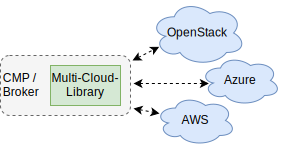
\includegraphics[width=0.48\textwidth]{images/multi-cloud-library.pdf}
	\def\svgwidth{0.75\textwidth}
	{\footnotesize \textsf{
			\includesvg{images/hyrise-r-deployment}}}
	\caption{Testarchitektur mit zwei Hyrise-R-Clustern, verteilt auf eine Public- und eine Private-Cloud. Cluster \emph{B} nutzt AWS, um unkritische Daten kostengünstig auszulagern. Orchestriert werden beide Services durch die selbst entwickelte Cloud-Management-Plattform aus der Private-Cloud heraus -- die CMP harmonisiert Provider- und Infrastrukturgefälle.}	
	\label{fig:hyrise-r-deployment}
	%\end{wrapfigure}
\end{figure}

Wir starten Hyrise-R immer als Cluster aus Dispatcher, Master und einer per SLO-Template bestimmten Anzahl an Replicas. Anschließend skalieren wir den Cluster dynamisch nach Leistungsanforderungen und SLO-Bedingungen. Das Re-deployment anhand von veränderter Umgebung ist eingeschränkt: Hyrise-R unterstützt keine Live-Migration. Einzig die Replicas lassen sich ohne Probleme an- und abmelden -- für Tests des Cloud-Burstings, also dem Abfangen erhöhter Last durch weitere Instanzen, ist das kein Problem: Entweder der Broker sucht eine passende Infrastruktur und startet einen neuen Hyrise-R-Replica-Knoten, oder er fährt einen Knoten herunter und meldet ihn ab. Die Tests sind rein qualitativ und decken folgende Fälle ab:

\begin{enumerate}
	\item Betrieb über Cloud-Grenzen hinweg
	\item Betrieb auf heterogener Infrastruktur
	\item Skalieren nach Leistungsanforderungen
	\item Skalieren nach weiteren SLOs und Nutzeranforderungen
\end{enumerate}

\todo{Tabelle der Testfälle}

In einem funktionsfähigen Hyrise-R-Cluster empfängt der Dispatcher alle Anfragen. Jede Anfrage mit Schreibanteil leitet er an den Master-Knoten. Hier wird die Anfrage bearbeitet, in das Log geschrieben und anschließend mit allen Replicas synchronisiert. Enthält eine Anfrage nur Leseanteile, verteilt der Dispatcher sie an einen beliebigen Knoten. Frühere Arbeiten bewerteten an dieser Stelle die Anfrageperformance und den Synchronisationsoverhead. Beide Metriken sind jedoch stark abhängig von der Performance der Cloud-Infrastruktur und Netzwerkverbindungen.

Als Metrik zur Bewertung des Brokerings gilt -- neben Einhaltung der SLOs -- die volle Funktionsfähigkeit des Clusters. Eine Beispieldatenbank ist bereits in den Images enthalten. Alle Anfragen haben ausschließlich lesende Anteile, die Tabelle wird nicht durch Schreibanfragen verändert und muss deshalb nicht synchronisiert werden. Gemessen wird also nicht die Synchronisationszeit der Hyrise-R-Lösung, sondern die Skalierungsfähigkeiten der verwendeten Cloud-Lösungen und Orchestrierungstechniken.

Die Hyrise-HTTP-Schnittstelle empfängt Anfragen im JSON-Format. Die minimale Anfrage \emph{NoOp} startet keine Datenbankoperation, durchläuft aber alle Datenbankkomponenten von HTTP-Handling über Parser bis Ausführungseinheit. Als erster Funktionstest würde diese Anfrage genügen. Wir möchten allerdings den gesamten Cluster testen, und nutzen daher eine echte, hinreichend komplexe Anfrage. Deren Bearbeitung benötigt genug Zeit, damit der Dispatcher sie auf alle Knoten aufteilen kann. Den vorhandenen Python-Code überarbeiten und parallelisieren wir. Die Anzahl der Knoten lässt eine bestimmte Performance erwarten -- für einen gültigen Test muss die Anzahl der Anfragen mindestens der Anzahl Knoten entsprechen:

\begin{minted}{python3}
queries = [(host, port, query)] * num_nodes
start_time = time.time()
with multiprocessing.dummy.Pool(num_threads) as pool:
	pool.starmap(query_hyrise, queries)
queries_second = num_nodes / (time.time() - start_time)
\end{minted}

Um sowohl OLTP- als auch OLAP-Fähigkeiten der In-Memory-Datenbank zu überprüfen, nutzen vorherige Arbeiten \cite{ssiclops:d42:experiments-measurements} den CH-benCHmark der TU München \cite{cole:2011:db-benchmark}. Dieser ist eine Mischung aus Transaktions- und Analysebenchmark, angelehnt an den hybriden Einsatz aktueller Datenbanksysteme in Unternehmen: Die gleichen Tabellen eines einzigen Datenbanksystems erfüllen alle Aufgaben des täglichen Geschäfts und liefern gleichzeitig umfassende Analysen. Trotzdem bleibt die Vergleichbarkeit des Benchmarks mit klassischen, getrennten Systemen.

Die Beispieldatenbank enthält eine Auftragshistorie mit knapp 300\,000 Datensätzen. Jede Zeile besteht aus sieben zufälligen Integer-, zwei String- und einem Float-Wert. So ergibt sich eine Rohgröße von 21,3\,MB. Die folgende Beispielanfrage\footnote{\url{https://db.in.tum.de/research/projects/CHbenCHmark/}} zeigt alle Bestellungen eines bestimmten Zeitraumes, sowie Summe, Gesamt- und Durchschnittswert aller enthaltenen Posten. Sie dient uns als \emph{Smoke-Test} -- liefert der Hyrise-R-Cluster eine valide Antwort im vorgegebenen Zeitrahmen, ist die generelle Funktionsfähigkeit gegeben, und das Deployment erfolgreich abgeschlossen:

\begin{minted}{sql}
SELECT ol_number,
       SUM(ol_quantity) AS sum_qty,
       SUM(ol_amount)   AS sum_amount,
       AVG(ol_quantity) AS avg_qty,
       AVG(ol_amount)   AS avg_amount,
       COUNT(*)         AS count_order
FROM orderline 
WHERE ol_delivery_d > '2007-01-02 00:00:00.000000' 
GROUP BY ol_number
ORDER BY ol_number
\end{minted}

To-do: Konkreter Test, SLOs: Verlinken aus vorherigem Abschnitt. Forschungshypothese: Steigerung von  Datensicherheit, Vertraulichkeit und Portabilität.

\section{Diskussion}

\todo{Mit Fazit zusammenlegen?}

%verschiedene OpenStack-Versionen haben unterschiedliche Schnittstellen. Auch dies kann über die Middleware abgefangen werden. RefStack testet API, Rally testet performance und führt tempest-Tests aus.


Aufwand einer Multi-Cloud-Strategie

Umsetzung der Policys

Potenzial

Vorteile durch Multi-Cloud-Bibliotheken

Aufwand für ein Multi-Cloud-Testbed

Redundanz fehlt: Auch die CMP muss in einer vertrauenswürdigen Umgebung repliziert werden und synchronisieren. Dem Hyrise-R-Dispatcher fehlt diese Funktion ebenso.